\chapter{State of the Art} \label{state_of_the_art}
This chapter will cover scientific work regarding the usage and application of UGC, comparisons of different data-sources, nature-based recreation as well as existing text-classification models. According to the presented current state of the art the research gap this thesis tries to fill is displayed and put into context.

\section{Applications of UGC} \label{applications_UGC}
The following subsections provides a general overview of the wide scientific spectrum for which UGC or more specifically VGI and social media data have been used.

\subsection{Quantifying ecosystem services}
Ecosystem services (ES) describe nature given benefits which are provided by functioning environments and their incorporated ecosystems \parencite{Jacobs2014}. Due to the complexity and intangibility of ES their associated (monetary) value is hard to estimate \parencite{ACostanza1997}. The value of \textit{provisioning} ES for instance such as 'clean water provision' can be estimated by calculating the water purification cost by state-of-the-art filter machines \parencite{Africa2018}. The potential value of \textit{cultural} ES such as the aesthetic value of landscapes is harder to grasp since it depends on the individual benefit people associate with it \parencite{Hunziker1995}. Through UGC - in particular in the form of social media data - people express their personal perception which has been used for the subsequent papers to estimate values of specific ES also as alternative to conventional methods such as interviews and surveys. \\

\textcite{Richards2018} applied similarly to this thesis the \textit{Google Cloud Vision} image recognition algorithm to 20'000 retrieved geo-tagged Flickr photographs of Singapore. The paper proposed the use of said photographs for the mapping of the cultural use or appreciation of ecosystems by automating the image content analysis process. Grouping by hierarchical clustering revealed that more than 20\% of the images were taken of nature, more precisely of animals and plants which were located dominantly around specific natural attractions, parks or generally areas with high vegetation cover. The approach developed by the paper is accurate and saved an estimated 170 hours of human image content analysis. As summary, the method provided by \textcite{Richards2018} allows the scalable mapping and assessment of cultural ecosystems services which can be easily applied to different areas of interest. \\

\textcite{Figueroa-Alfaro2017} used geo-tagged photographs from Flickr and \\ Panoramio\footnote{https://www.panoramio.com/, out of service since 04.11.2016} as a type of crowed-sourced alternative to traditional methods to examine the relationship between the aesthetic value of landscapes and locations where citizens' perform nature-based activities in Nebraska. The Flickr API was queried with 26 keywords that relate to natural resources with the potential for aesthetic value (e.g. wetland and waterfall) which resulted in 19'221 images. Panoramio was designed to be a photo-sharing platform that hosts non-commerical and mostly nature related content. To enforce these rules, every uploaded image must fulfill the 'acceptance policy for Panoramio photos' of Google which is checked by a dedicated filter. Therefore, the Panoramio API was not queried specifically but rather all 1'967 available images of the region were retrieved.\\
The outcome of the spatial clustering of the photographs with the cluster/ outlier analysis tool\footnote{https://pro.arcgis.com/en/pro-app/tool-reference/spatial-statistics/cluster-and-outlier-analysis-anselin-local-moran-s.htm, accessed: 03.04.2019} from ArcGIS that applied Anselin Local Moran's I statistic, identified existing and new areas with aesthetic value at a 95\% confidence level. \citeauthor{Figueroa-Alfaro2017} underlined the importance of the findings also for urban planning and environmental management. Knowing which areas people prefer to visit helps to allocate available resources more efficiently and supports the preservation as well as conservation of natural resources from which simultaneously the local tourism profits. \\
\newline
A similar study was performed by \textcite{Yoshimura2017} that made use of viewsheds of geo-tagged Flickr photographs of Hokkaido, Japan. \citeauthor{Yoshimura2017} proposed that areas with many overlapping viewsheds represent areas of high aesthetic and therefore cultural value since they were the focus of many visitors. Detecting the photographic orientation as already proclaimed by \textcite{Unknown2013} was problematic. Also the overestimation of popular and highly visited sites was recorded as potential bias which is reflected in the resulting areas of interest mapping.


\subsection{Visitor rates \& monitoring}
Good management and marketing relies heavily on customer information. The same applies to the environmental management of recreation sites, protected or conservation areas \parencite{Ralf1991}. Detailed knowledge about the visitors from which the projects live is key. The following papers will present data-acquisition approaches to answer questions related to visitor behaviour. \\  

\textcite{Heikinheimo2017} used the most popular national park named Pallas-Yll\"astunturi in Finland as research area to investigated visitor behaviour. This encompassed the identification of sub-areas in the park with the highest visitation rates, spatial and temporal patterns of performed activities, reasons for visit and information about the demography as well as home location of visitors. The data to answer those questions was collected through 1'927 visitor surveys and 19'939 geo-tagged Instagram images from 7'700 unique users. The aim of this two sided approach was to test to what extent social media content reflects or complements the reported experiences extracted from the traditional methods. This controversy is further elaborated in section \ref{data_comparison_SotA}. The data-comparison and research questions of \textcite{Heikinheimo2017} are comparable to this thesis but the applied methods differ.
The highly visited areas were identified according to the spatial density distribution of the geo-tagged Instagram images. These images were manually classified according to the performed activities where displayed equipment played an important role. Potential home location of 291 Instagram users that visited the park were detected by analysing the country or region from which the most photos were uploaded. \\
The results revealed that social media platforms are a potential source for continuous visitor monitoring as a rapid and cost-efficient alternative to traditional surveys. With the help of the social media data it was possible to detect the most popular sub-regions of the park. Also, the Instagram data revealed performed activities that were not captured by the survey. Walking and hiking had the highest recorded occurrence according to both data-sources which corresponds to the findings of this thesis. Lastly, \textcite[p.10]{Heikinheimo2017} proclaims potential for "using Instagram photographs for group-size estimation for small to medium sized groups (2-10 people), but not necessarily for detecting people travelling alone or in very large groups." \\

\textcite{Pettersson2011} examined the usage of GPS-data as 'crowdsensing' data-foundation to understand the time and space movement of visitors to the Biathlon World Championships 2008 in \"Ostersund, Sweden. In addition to equipping people with GPS-devices which additionally enabled them to input personal experiences to a certain location, questionnaires were used to study the visitors movements and experiences also. The aim of the study was to evaluate the practicability of GPS-data during an outdoor sport event. \\
The results of the paper allowed for a comparison of the strengths and weaknesses of the UGC and the questionnaire data which suggested a combination of both methods to yield the best information retrieval. In conclusion, the usage of crowdsourced GPS-data was successful to grasp the macro-movements and experiences of the visitors. This paper provides a good transition to research that tries to quantify bigger-scale movements of people in space.

\subsection{Mobility patterns}
The mobility of people is an highly valued necessity. Correspondingly, the planing and optimisation of transportation systems such as road and rail nets especially in urban areas is important. \\

\textcite{Barchiesi2015} derived mobility-patterns for the UK using a machine learning algorithm trained on 8 million geo-tagged images of 16'000 individual Flickr users between 2007 and 2013. The model is capable of inferring the probability of people being in a certain location as well as the probability of trajectory-movement between different locations. Considering Flickr-data as a proxy for human mobility comes with the limitation that pictures from the same user with long time-spawns between them potentially lead to false or incomplete travel-pathways. \textcite[p.7]{Barchiesi2015} were able to show that this issue is mitigated by the fact "that the time elapsed between consecutive photos follows a heavy tailed distribution [\dots] with most photos taken only a few hours or a few days apart, and only a small number of photos taken as much as a few years apart." \\
The paper concludes that there is fundamental evidence that Flickr derived data can be used to quantify human mobility. Due to a lack of official survey data the presented model could only be partially validated but they appear to be in general agreement. \\

\textcite{Grossenbacher2014} conducted an commuter mobility-analysis for entire Switzerland. 1 year worth of geo-tagged Twitter\footnote{https://twitter.com/, accessed: 01.04.2019} posts were used as data-foundation to extract transportation flows between major cities. An intensive literature review revealed flaws of preceding work. \citeauthor[p.5]{Grossenbacher2014} points out that often times mobility-patterns were inferred from "mere spatial aggregations of individually unreferenced, decoupled content." Correspondingly, the thesis presented an approach of linking Twitter users to specific municipalities inside of Switzerland while estimating home and work locations. This in conjunction with a sophisticated pre-processing of the data enabled the comparison of the results to official data.\\
The conclusion states that Twitter-data hints at a "socially, culturally, and economically unequally represented population, which raises concerns about the validity of inferences made with such data." \parencite[p.4]{Grossenbacher2014} Nevertheless it can be used as a potential data-source for studying human-mobility since it provides good indicators for actual flows of people in regions where sufficient geo-tagged data is available.

\subsection{Disease outbreak tracking}
Infectious disease epidemiology has recognised big data such as UGC as novel potential sources to complement traditional infectious disease surveillance. The real-time data-acquisition with included locational information from multiple data-streams could allow for spatially broader predictions and would help formulate future disease-mitigation strategies. Additionally, determining origins of epidemic outbreaks as well as identifying locations with risk of new outbreaks are tasks for which UGC holds possible answers. The following papers list concrete sources of UGC and critically discuss their incorporated biases when used for disease surveillance.\\

Crowed-sourced data with locational information in some form is essential. According to \textcite{Lee2016, Schmidt2012} there are several options that emerged with the phenomenon of the internet that hold potential. People entering their symptoms into a search engine such as Google allows for approximations of their location based on their assigned Internet Protocol (IP) address. Google hosted a Flue Trend project\footnote{https://www.google.org/flutrends/about/, accessed: 02.04.2019} from 2008 until 2014 which used their search statistics to predict flu outbreaks. The related country specific data is still accessible but the service has been retired. The topic and potential of mobile data has not yet been touched upon in this thesis but will be shortly mentioned here. 
Cellular data is linked to known cell-tower locations to which a mobile device connected. Mobile providers log this information which holds activity and mobility patterns that can be mapped to a specific person according to the used SIM-card. This data has provided insights into human mobility that have informed risk maps, importation potential, and spatial dynamics of dengue and malaria. \parencite{Buckee2015b} \\
Reservation cancellations to restaurants over websites like OpenTable\footnote{https://www.opentable.de/, accessed: 02.04.2019} or the shopping activity for pharmaceutical goods in drug stores as well as in online shops could be a proxy for the emergence of illnesses. Geo-tagged social media data (e.g. Twitter, Facebook, Instagram) where people online share details about their wellbeing is also mentioned. Both papers point out that aggregations of different data-streams which led to tools such as HealthMap\footnote{https://www.healthmap.org/en/, accessed: 02.04.2019} bring together the benefits and partially mitigate the bias incorporated in all of them.\\
The encountered challenges and biases are similar to general social media data applications which encompass incomplete and unrepresented populations as well as invalidated data. Additionally, the usage of sensitive health related data raises many ethical issues. \textcite{DeMontjoye2013} have shown that presumably anonymised data could be de-anonymised by linking it to certain available databases. Considering health insurances, leakage of said personalised data could have shrouded consequences for the individuals involved.  
\textcite[p.410]{Lee2016} concludes: "[\dots] there remain untapped opportunities with real-time surveillance, large-scale ecological inference, and adaptive disease mitigation strategies. Harnessing disease data from digital sources may enable epidemiological analyses to be performed at finer spatial scales in areas with poor coverage from traditional public health surveillance [\dots]".

\section{Data-comparison} \label{data_comparison_SotA}
Several of the presented papers that worked with UGC compared their results to empirical data for data-validation and for prove of legitimacy. Additionally, it is necessary to comprehend and compare biases, strengths and weaknesses from different sources of UGC to find the most well-fitting data for a certain application. The following literature provides the results to said comparisons in further detail.

\subsection{Data from different social media platforms} \label{SMP_vs_SMP}

\textcite{Tenkanen2017} addressed the issue that most studies that analysed recreational use have relied on data from a single social media platform. Correspondingly, the popular social media platforms Instagram, Twitter and Flickr were used to investigate how well they individually or in combination predict visitation rates in 56 national parks in Finland and South Africa. High-precision visitor statistics from the year 2014 were available from these parks which additionally allowed for evaluating the use of social media data as proxy for visitation rates and identifying popular attractions.\\
Figure \ref{fig:tenkanen_SMP} shows the results of the study. The numerical acquired visitation rates allowed for a popularity ranking of the 52 national parks which were compared to the ranking derived from the three individual social media platforms and them in combination. The Spearman's rank order correlation of 0.75 in South Africa and 0.84 in Finland revealed that the social media data matches the official ranking well. There are apparent accuracy differences between the two countries and between individual social media platform's. Instagram managed to correctly predict the top four of the 21 South African national parks whereas Twitter only managed to correctly predict the top two. The results for the 35 national parks located in Finland showed more variation in the top ranks but were able to approximate better to the general order.

\begin{figure}[h]
   \centering
   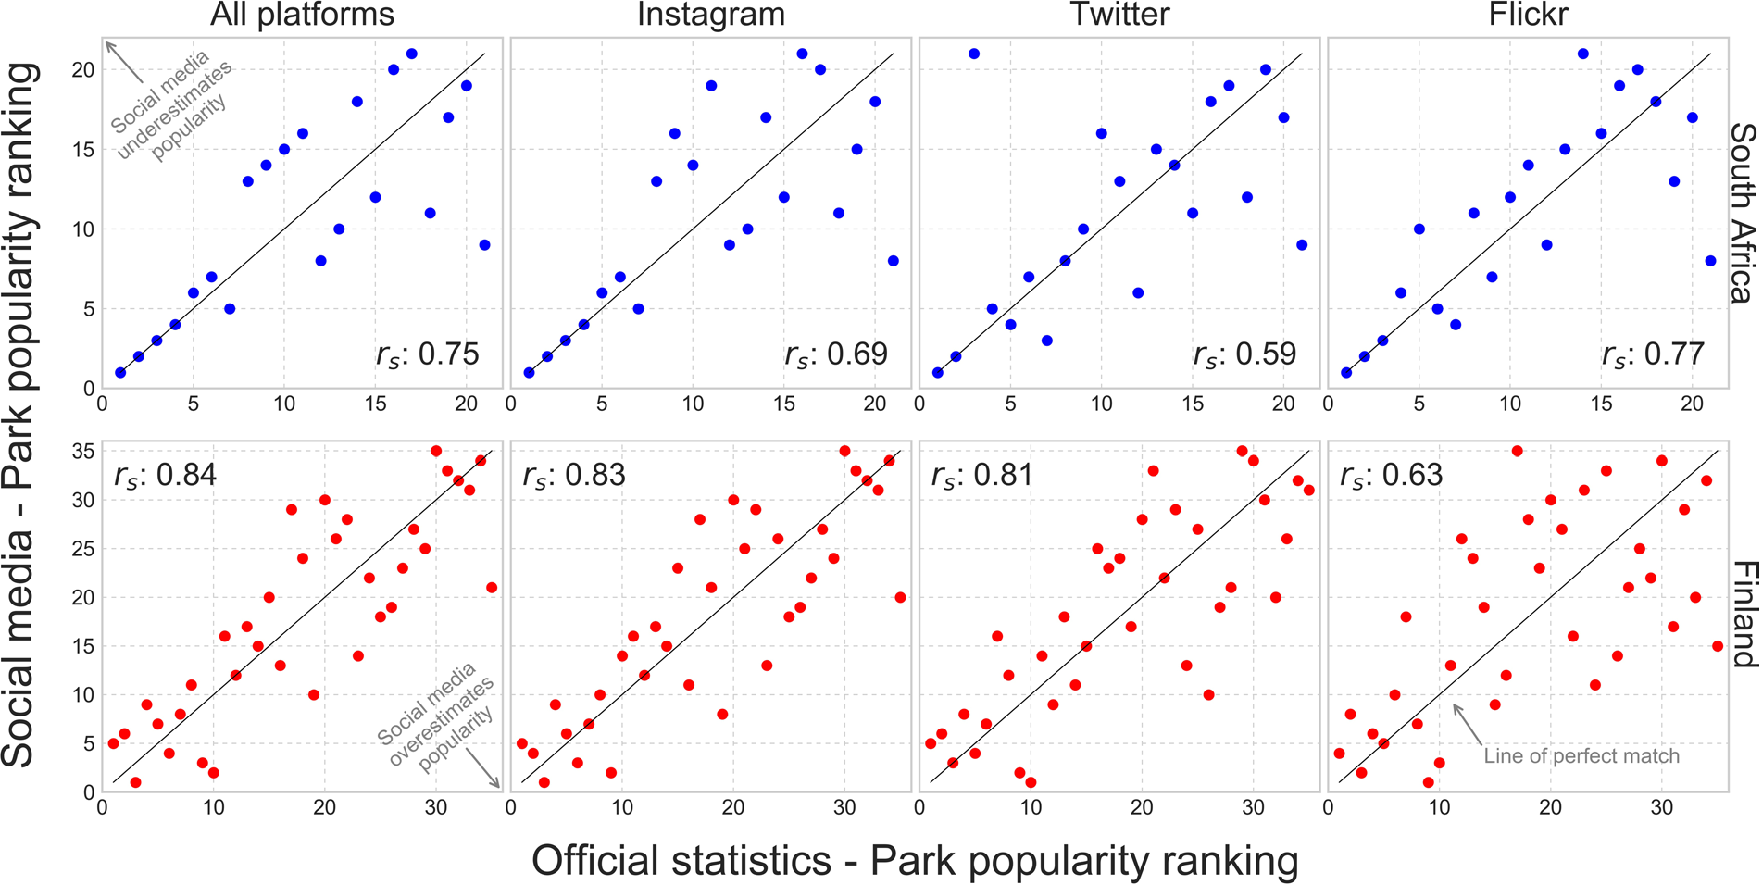
\includegraphics[width=\textwidth]{img/tenkanen_2017_SMPs.pdf}
   \caption{Shown are the park rankings inferred from the social media platforms Instagram, Twitter and Flickr compared to the official visitor statistics of the 21 and 35 national parks from South Africa and Finland respectively. Source: \textcite[p.4]{Tenkanen2017}}
   \label{fig:tenkanen_SMP}
\end{figure}

\textcite{Tenkanen2017} identified together with involved stakeholders potential explanations for certain mismatches in the data. In summary, the geography and profile of the park, the visitor profile, and sudden events were mentioned as possible reasons.\\
The paper concludes that fusions of different data-streams hold the potential to describe patterns in the data more thoroughly than on their own. This is mainly due to the fact that people use multiple social media platforms simultaneously. Merging these channels allows to capture the bigger picture.
It was shown that "[\dots] social media activity is highly associated with park popularity, and social media based monthly visitation patterns match relatively well with the official visitor counts. However, there were considerable differences between platforms as Instagram clearly outperformed Twitter and Flickr."\parencite[p.1]{Tenkanen2017}

\subsection{UGC versus empirical data} \label{ugc_vs_empirical}
Section \ref{applications_UGC} presented the application-broadness of UGC. The question arises how well this data and the therefrom drawn conclusion represent reality. Empirical data is considered to be the closest approximation to reality. This section will introduce papers which investigate the legitimacy of UGC (specifically social media data) as proxy for real world conditions compared to empirical data acquired through conventional methods such as interviews and surveys. \\

\textcite{Wood2013} examined the Flickr data in particular and its ability to predict among others visitation rates to 836 recreational sites located in 31 countries around the world. Through the official Flickr API (see \nameref{definitions}) metadata of images inside the site-boundaries were acquired which consisted of the location, the date the image was taken and the author id which was additionally used to estimate the visitors origin. The measurement used to compare the empirical visitation rates to the Flickr data was the so called \textit{User-Days per Year}. It was calculated by looking at every individual Flickr author (according to the author id) that ever uploaded pictures inside one of the considered recreational sites. According to the upload-dates of the media objects the length of the visits inside the sites were estimated. The user-days are the sum of all days spent inside the site aggregated over all authors. Normalised over the years this measurement is assumed to correlate with empirically estimated visitation rates. \\
Figure \ref{fig:wood_user_days} shows the comparison of these two measurements. Even though they do not resemble a 1:1 relationship as indicated by the grey line, a linear correlation can be assumed. The paper concludes that "the crowd-sourced information can indeed serve as a reliable proxy for empirical visitation rates." \parencite[p.1]{Wood2013}

\begin{figure}[h]
   \begin{center}
   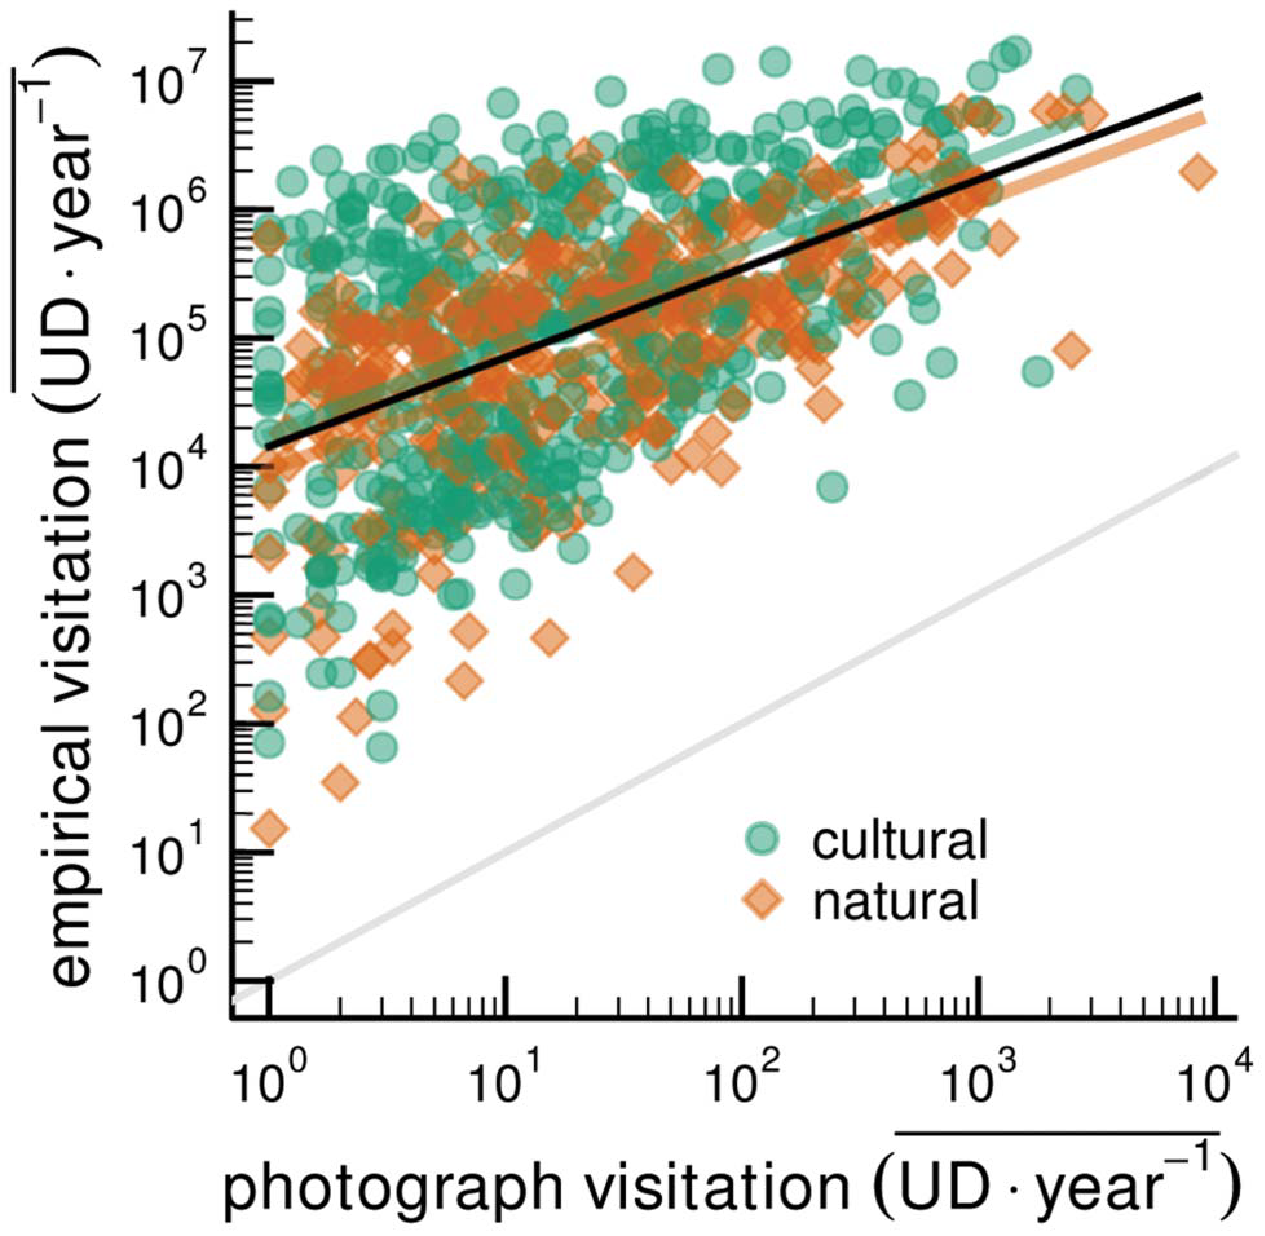
\includegraphics[width=0.49\textwidth]{img/wood_user_photodays.pdf}
   \end{center}
   \caption{Relationship between the user-days per year and the empirical visitation rates of both cultural (green circle, \textit{n}=498) and natural (orange diamond, \textit{n}=338) recreational sites. Source: \textcite[p.4]{Wood2013}}
   \label{fig:wood_user_days}
\end{figure}

\textcite{Wartmann2018} compared three different data-sources according to extracted landscape descriptions from five landscape types. The considered data-sources were free-lists, crawled website-content and geo-referenced Flickr images. A total of 10 study sites located in Switzerland were queried. The free lists were generated by asking 30 people per study site to list landscape elements they personally find distinctive or striking. The web-crawled corpora containing text-descriptions about landscapes and the associated experiences were generated with the open-source tool BootCaT \parencite{Baroni2004} which was fed location-specific toponyms as well as the German word for 'hiking' (wandern) and 'we' (wir). This method yielded between 40 and 70 webpages per study site. Lastly, Flickr images were queried for a spatial perimeter that was inferred from the extracted toponyms accociated with every study site. The relation between toponyms and coordinates was achieved through the GeoAdmin API\footnote{http://api3.geo.admin.ch/, accessed: 02.04.2019} which accesses the SwissNames3D gazetteer. The landscape descriptions of the three data-sources and the five landscape types were compared using cosine similarity. \\ 
The results of the study show that landscape description from the same data-source were significantly more similar independent of landscape type. Also, descriptions from the same landscape type were more similar within each considered data-source. Consequently, the data-sources exhibit considerable differences according to the low cosine similarities.


\section{Nature-based recreational assessments}
%The terms nature-based recreation, outdoor recreation or soft ecotourism \parencite{Deng2002} are associated with activities such as cycling, hiking, horse riding and wildlife watching. The provision of nature-based recreation is considered to be a cultural ecosystem services with potentially high monetary value. \textcite{Shrestha2007} showed with the travel-cost method that people were willing to pay on average \$74.18 per visiting-day for nature-based recreation in the Apalachicola River region of Florida. 
%The spatial mapping of recreational activities becomes increasingly important with growing use intensity. Uncontrolled and excessive land encroachment can be damaging to nature and the biodiversity \parencite{Song2018}.
%Additionally, the allocation of supporting assets such as infrastructure requires location-based information about people's usage of space for spatial planing agencies to operate efficiently \parencite{Sen2014}.

\subsection{Using empirical data from conventional methods}

\textcite{Weyland2014} evaluated and mapped the outdoor recreation potential as a cultural ecosystem service in the country Argentina. The Ecosystem Services (ES) framework is used to estimate the ecosystem service supply and benefit of different landscapes. The approach considers nine landscape metrics such as land cover (share of crop, forest and bare soil area) and biophysical measurements (among others: mean annual temperature, NDVI\footnote{Normalised Difference Vegetation Index as an indicator of dense vegetation} and coastal density) at a coarse as well as campsite scale for 10 typical ecoregions of Argentina. Land use related factors were not specifically considered. \\
The results revealed that the examined landscapes differ in their capacity of outdoor recreation potential. Crop area mostly accounted for positive correlations on the capacity of outdoor recreation potential contrary to forest cover. Also road and population density were proven to show for higher benefits. \\

\textcite{Sen2014} present a general tool for recreational planning and environmental decision making since 2'858 million outdoor recreational visits were made in England during 2010, entailing direct expenditure of over $£$20 billion. Therefore, a spatially sensitive prediction of outdoor recreational visits and values for different ecosystems in the United Kingdom was conducted. Their data-foundation consisted of outset and destination characteristics and locations combined with survey information from over 40'000 households. This data was used to create a trip generation function to predict visitation numbers and their associated values.\\
The result provided by the Geographic Information System (GIS) powered tool showed the importance of travel and time costs, site characteristics, substitute availability and socioeconomic and demographic factors in determining the pattern and level of recreational demand. \\

\textcite{Neuvonen2010} investigates the relationship between the number of visits to 35 national parks in Finland and their characteristics via linear regression modelling. The understanding of these relationships is crucial for park planing and management to understand what draws people to certain areas. Considered were the natural characteristics such as the dominant natural features (water areas, mires, fells or forest), the recreational facilities (shelters, viewing towers and campfire sites), services inside a park and tourist services (e.g. events) in surrounding communities. The latter were collected from unspecified internet sources.\\
The results of the study revealed that the variety of recreational opportunities, the number of biotopes, the provision of trails and the park's age increase the number of visits. It was also shown that parks located close to populated areas dominantly fulfil recreation-provision services over simply being resource-based destinations.

\subsection{Using UGC} 

\textcite{Monkman2018} used social media mining to acquire crowed-sourced spatio-temporal information about fishery in Wales as a wildlife recreational activity. Details about fish size and fisher activity (crew size, trip duration and route) were geo-referenced using a custom gazetteer to match extracted toponyms. The data consisted of 10'000 blog posts from a total of eight relevant forums regarding fishery in Wales. These extracted URLs were mined through automated web-scraping using Outwit Hub\footnote{https://www.outwit.com/products/hub/, accessed: 03.04.2019} which was ethically acceptable given users dominantly used pseudonymous. Subsequently, the data was analysed and categorised using a text-classification algorithm to identify posts among others related to catch measurements, used equipment, trip duration, trip route and the used vessel. This information was extracted together with the geo-referenced toponyms to map the activity. \\
The results of the study indicate that crowed-sourced data such as blogs can be used to unveil spatial and temporal patterns related to wildlife recreation since the predicted occurrences and intensities of fishery in Wales agreed qualitatively with expert knowledge. \\

\textcite{Mancini2018} focused on identifying nature-based recreational hotspots in Scotland, specifically of wildlife watching of birds, seals, whales and dolphins for which Flickr data was used. Additionally, comparisons to empirical numbers were conducted to backup their findings and legitimise the usage of Flickr as indicator for spatial and temporal dynamics of nature-based recreational activities.
Two separate Flickr datasets were acquired. The first one contained a monthly time-series of Flickr photographs taken inside the Cairngorms National Park between 2009 and 2014 which was compared to an official visitor statistic. The second dataset contained Flickr photographs from the Scottish coastline between October 2014 and October 2015 to identify the mentioned wildlife watching hotspots of dominantly marine animals. The keywords 'bird', 'seal', 'dolphin' and 'whale' were used to query the official Flickr API. This data was correspondingly compared to a spatial dataset of wildlife watching from the Scottish marine recreation and tourism survey \parencite{LUC2016}. \\
The generated output assumes the existence of reliable statistical accordance between short-term and seasonal patterns of Flickr data and temporal visitation patterns to the Cairngorms National Park.  
Also, the identified wildlife watching hotspots match with the recreation and tourism survey data down to a spatial resolution of 10km. The temporal pattern analysis additionally confirmed seasonal movement towards these areas. \textcite{Mancini2018} concludes that Flickr (and potentially other crowed-sensing sources) holds the potential to identify people's preferences and movement which could be used to e.g. monitor the pressure recreational activities impose on the environment.

\section{Existing text-classification models}\label{existing_text_class_models}
In the current time, text-classification is implemented in a variety of different software systems that deal with text-data at scale and is a fundamental component to the majority of natural language processing as well as machine learning use cases. A common application of text-classification models are SPAM-filters that classify e-mail content according the usefulness to the owner. Sentiment analysis, topic labelling and language as well as intend detection are other frequent applications\footnote{https://monkeylearn.com/text-classification/, accessed: 07.04.2019}.\\
The following two papers present modern comforts of text-classifications models based on machine learning and deep learning. The aim of this section is not to explain certain fitting algorithms or deep-learning concepts, but moreover give a short overview of existing models and the performances they yield. The performances of the following two models will be used as baseline. Comparisons to the models of this thesis will be presented in the \nameref{discussion} chapter under section '\nameref{model_baseline}'. \\

\textcite{Das2018} attempted to improve traditional TF-IDF\footnote{Term Frequency times Inverse Document Frequency, see also \nameref{definitions}} bag-of-words models by implementing Next Word Negation (NWN). Next word negation is an algorithm developed by \textcite{Das2018} which aims to identify forms of negation inside a document corpus. This procedure differs from similar algorithms by negating only the very next word after an identified negation word instead of all preceding words until a punctuation is received. The presented model aims to predict text sentiment on three different datasets with three tested classifiers. Movie reviews, product reviews and SMS\footnote{Short Message Service} spam excerpts were used as individual datasets for training and testing with an split ration of 0.8 (80\% of the data for training, 20\%  for testing). Multinomial Na\"ive Bayes, Max Entropy Random Forest and Linear Support Vector Machines are popular algorithm choices for text-classification whose performances were evaluated on the datasets. \\
The result show that the implemented NWN is able to improve model performance. The Linear Support Vector Machine classifier performed the best with 10-fold cross-validated accuracies on the IMDB movie reviews, Amazon product reviews and SMS spam detection dataset of 89.91\%, 96.83\%, 88.58\% respectively. \\

\textcite{Li2018} proposed a new hybrid deep-learning model by combining layers of Long Short-Term Memory (LSTM) and Convolutional Neural Network's (CNN) to classify Chinese and English text of being either tech, sports, politics, entertainment or business. LSTM is capable of processing serialised information while CNN excels in feature extraction. The combination of these methods resulted in the novel BLSTM-C model whereby BLSTM stands for Bi-Directional Long Short-Term Memory while C stands for CNN. The model-hybrid was tested on the Stanford Sentiment Treebank benchmark (SST-1) from \textcite{Socher2013} which is made up of 11'855 movie reviews of which 8'544 (72\%) were used for training, 1101 (9\%) for validation and 2'210 (19\%) for testing. \\The results revealed an BLSTM-C model accuracy
of 94.88\% on the English dataset and 96.23\% on the Chinese dataset. This corresponds to an respective improvement of 3.15\% and 5.12\% compared to the simple LSTM model.

%\textbf{Disclaimer:} The author of this thesis is not familiar with the exact workings behind the mentioned deep-learning concepts. The paper was merely chosen from the field of neural networks for comparison reasons.

\section{Research gap}
According to the presented scientific advances in the field of nature-based recreation as a cultural ES and the spectrum of applications of crowed-sourced UGC, the research gap this thesis tries to fill will be illustrated. \\
Previous research harnessed either text-data \parencite{Barchiesi2015, Monkman2018, Wartmann2018} or image contained information \parencite{Richards2018, Heikinheimo2017} from various UGC-sources. Rarely have the two data-streams efficiently been combined to yield potentially more precise predictions of real world circumstances. This thesis tries to accomplish the synthesis of these two data-sources in the form of a sophisticated text-classification model which is trained on processed user-generated text-data and structural elements contained in images of social media posts. The model is used to map the spatial occurrences of NBRAs based on data from two different social media platforms Instagram and Flickr. The social media platform specific bias in the data such as the asymmetric representation of the population can thereby be partially mitigated opposed to relying on a single data-source \parencite{Barchiesi2015, Grossenbacher2014, Monkman2018, Mancini2018}. \\
The approach brings innovation by automating the identification process of NBRAs in UGC. The use of the Google Cloud Vision image recognition algorithm omits expensive labour needed for manual image classification as shown by \textcite{Richards2018}. Additionally, the model can be rapidly applied to new study areas and allows modifications such as the implementation of new classes. The approach's repeatability is assured since dominantly Open Source or free software was used which reduces license costs and simultaneously increases the benefit for small agencies. \\
Lastly, the acquisition of \textit{in-situ} ground truth data allowed to overall substantiate this thesis' findings and provide further insight on the proxy potential of social media data compared to conventional methods. 

 